% Template for PLoS
% Version 1.0 January 2009
%
% To compile to pdf, run:
% latex plos.template
% bibtex plos.template
% latex plos.template
% latex plos.template
% dvipdf plos.template

\documentclass[12pt]{article}
%\usepackage{amsmath}
%\usepackage{lineno}
%\linenumbers
%\usepackage{mathtools}
%\usepackage{amssymb}
\usepackage{lscape}
\usepackage{color}
\usepackage{graphicx}
\usepackage{times}
\usepackage{tikz}
%\usepackage{amsmath}
\usepackage{verbatim}
\usepackage{animate}
\usetikzlibrary{arrows,shapes}
\usepackage{cite}
\usepackage{color} 
\usepackage{longtable}
\usepackage{setspace}
\usepackage{caption} \captionsetup[table]{singlelinecheck=false}
%\usepackage{natbib}

\doublespacing

% Text layout
\topmargin 0.0cm
\oddsidemargin 0.5cm
\evensidemargin 0.5cm
\textwidth 16cm 
\textheight 21cm

% Defining table column space
\setlength{\tabcolsep}{12pt}

% Bold the 'Figure #' in the caption and separate it with a period
% Captions will be left justified
\usepackage[labelfont=bf,labelsep=period,justification=raggedright]{caption}

%Use the PLoS provided bibtex style
%\bibliographystyle{painphysician}
\bibliographystyle{rheumatology}

% Remove brackets from numbering in List of References
\makeatletter
\renewcommand{\@biblabel}[1]{\quad#1.}
\makeatother

% Leave date blank
\date{}

\pagestyle{myheadings}

\begin{document}
\begin{flushleft}
\Large\textbf{Altered gait and balance in patients with fibromyalgia }\\\end{flushleft}
Isis da Silva Costa$^{1}$, Antoni Gamund\'i$^{1}$, Jos\'e Garcia Vivas Miranda$^{2}$, Lucas Gabriel Souza Fran\c{c}a$^{2}$, Charles Novaes de Santana$^{3}$, Pedro Montoya$^{1}$  
\\
\\
{\small $^{1}$ Research Institute on Health Sciences (IUNICS), University of the Balearic Islands, Palma de Mallorca, Spain
\\
$^{2}$ Department of Physics of the Earth and the Environment, Federal University of Bahia, Salvador, Brazil
\\
$^{3}$ Institute of Evolutionary Biology and Environmental Studies, University of Z\"urich, Z\"urich, Switzerland
\\
\\
\textbf{Corresponding author:} Pedro Montoya, pedro.montoya@uib.es }

%Corresponding author: Pedro Montoya, PhD, Research Institute of Health Sciences (IUNICS), University of Balearic Islands, Carretera de Valldemossa km 7.5, 07122 Palma, Spain. Phone: +34 971 172646. Fax: +34 971 259935. Email address: pedro.montoya@uib.es }}

% Please keep the abstract between 250 and 300 words
\section*{Abstract}
Fibromyalgia is a common chronic pain condition that exerts a considerable impact on patients' daily activities and quality of life. Objectives: The main objective of the present study was to evaluate the kinematic and kinetic parameters of gait, functional performance and balance in women with fibromyalgia syndrome. Methods: The study included 26 female patients with fibromyalgia ($49.2 \pm 8.0$ yrs) according to the criteria of the American College of Rheumatology, as well as 16 pain-free women ($43.5 \pm 8.5$ yrs). Gait and balance parameters were extracted from video recordings of participants performing several motor tasks. Non-linear dynamic of body sway time series was also analyzed by computing the Hurst exponent. In addition, subjective measures of motor function and clinical pain were obtained by using self-report questionnaires. Results: Walking speed was significantly diminished ($p < .001$) in FM patients as compared to pain-free controls, probably as result of significant reductions in stride length ($p < .001$) and cycle frequency ($p < .001$). Analyses of balance also revealed significant differences between fibromyalgia and pain-free controls on body sway in the medial-lateral and anterior-posterior axes (all $ps < .01$). Deficits in gait and balance were significantly associated with pain, fatigue, and stiffness in fibromyalgia, but not with depression or anxiety. Conclusion: Our analysis revealed that FM patients displayed balance and gait characteristics similar to those observed during aging processes. These results suggest that a precise evaluation of impairments and strategies underlying functional performance in postural stability and gait is necessary for optimal rehabilitation and fall prevention in fibromyalgia.\\
\textbf{Keywords}: Fibromyalgia; Pain; Gait; Balance; Biomechanics; Hurst Exponent


\section*{Introduction}
Fibromyalgia (FM) is a chronic syndrome characterized by widespread pain sensitivity and fatigue, as well as cognitive and affective symptoms \cite{wolfe2010american}. Fibromyalgia also exerts a considerable impact on daily activities and quality of life. In particular, it has been frequently shown that fatigue in fibromyalgia may be severe enough to reduce physical activities and lead to a sedentary lifestyle by reducing physical abilities and increasing risk for disabilities \cite{jones2008self, bennett2007internet}. FM patients often reported functional limitations that were quite similar to those reported by persons with osteoarthritis or rheumatoid arthritis \cite{hawley1991pain, meireles2014prevalence}. Furthermore, it has been shown that loss of function could be strongly associated with work disability in these patients \cite{white1999comparing, wolfe2004severe}. 

Previous research has also revealed that FM patients may also display deficits in balance or postural stability \cite{bennett2007internet, russek2009pilot, jones2009fibromyalgia}, a complex task that involves rapid and dynamic integration of multiple sensory, motor, and cognitive inputs to execute appropriate neuromuscular activity \cite{horak2006postural}. Impaired balance has been reported as one of the top ten debilitating symptoms in fibromyalgia with prevalence rates around 45\% \cite{bennett2007internet}. Moreover, frequency of falls seems to be higher in FM patients (34.4\%) \cite{russek2009pilot} than in persons aged 65 years and older (25-35\%) \cite{sattin1992falls}, and patients with rheumatoid arthritis (RA) \cite{meireles2014prevalence}. Nevertheless, balance and activity level in fibromyalgia have been mostly assessed by using retrospective self-reports \cite{russek2009pilot, mannerkorpi1994}, which are strongly influenced by patients' beliefs about their own physical functioning and pain \cite{verbunt2003disuse}. In the last decades, different types of recording devices have been developed to monitor and to assess balance and physical activity over long periods of times, providing valid information about subjects' daily activities. Thus, it has been demonstrated that accelerometry-based ambulatory monitoring systems provide more objective measurements of variability in physical activities and pain over several days than self-reports \cite{verbunt2009assessment}.

Biomechanical analysis of gait also constitutes a useful tool for the assessment of motor function, functional capacity and muscle fatigue \cite{pierrynowski2005women, bendtsen1997evidence}. Previous studies have observed that fibromyalgia women display a reduced walking speed, which could be a consequence of decreases in stride length and cycle frequency, as well as bradykinesia \cite{jimenez2009spatial, auvinet2006gait}. Furthermore, it has been suggested that gait at normal speed in these patients may be preferentially achieved by using their hip flexors instead of their ankle plantar flexors, thus increasing metabolic demands and fatigue in comparison to pain-free controls \cite{pierrynowski2005women}. 

The aim of the present study was to analyze gait and balance parameters in fibromyalgia and to examine the possible relationship between subjective and objective measures of motor function with subjective complaints. In particular, we hypothesized that FM patients would display significant gait and balance deficits as compared with pain-free controls, and that these motor disturbances would be associated with increased patients' ratings of pain, fatigue, morning tiredness, stiffness and physical impairment. Considering that activity and balance fluctuations have well defined fractal properties in the time scale of seconds to hours, we also aimed to apply nonlinear analyses to evaluate the dynamic of these balance fluctuations in pain-free controls and FM patients.\\

\section*{Material and Methods}
\emph{Participants}\\
Twenty-six women diagnosed with fibromyalgia (FM) and 16 pain-free women with comparable age and anthropometric characteristics (Table 1) were recruited from different health centers and patients' associations in Majorca (Spain). Patients were included in the study if they fulfilled the 1990 classification criteria of the American College of Rheumatology for fibromyalgia. Participants were excluded from the study if they reported any other musculoskeletal rather than fibromyalgia, or any neurological disorder. For medical and ethical reasons, subjects were asked to keep their medication during the study. At the time of recruitment, participants were verbally informed about the details of the study and provided written consent. The study was in accordance with the Declaration of Helsinki (1991) and was approved by the Ethics Committee of the Balearic Islands (Spain) (reference IB-1284/09).\\
\\
\emph{-- Tables 1 --}\\
\\
\emph{Self-report questionnaire}\\
FM patients completed the Fibromyalgia Impact Questionnaire (FIQ) \cite{burckhardt1991fibromyalgia}. The FIQ is a standardized instrument designed to quantify the overall impact of fibromyalgia over many dimensions (e.g. function, pain level, fatigue, sleep disturbance, psychological distress, etc.). This questionnaire has shown excellent responsiveness to change in clinical studies and a good correlation with other similar questionnaires, such as the SF-36 \cite{bennett2005fibromyalgia}.\\
\\
\emph{Motor function tasks}\\
Gait and balance parameters were obtained in FM patients and pain-free controls by using the following functional tasks:\\ 
\\
- \emph{Berg Balance Scale} \cite{berg1991measuring}: This scale is a performance-based assessment tool developed to measure balance during functional activities such as reaching, bending, transferring, and standing. The test is often used for patients who exhibit a decline in function, self-report a loss of balance, or have unexplained falls \cite{berg1991measuring}. The Berg Balance Scale consists of 14 functional tasks (e.g., sitting unsupported, change of sitting to standing position and vice-versa, standing with both feet together, standing on one leg, turning 360 degrees) with scores ranging from 0 (unable to perform) to 4 (normal performance). Total scores range from 0 (severely impaired balance) to 56 (excellent balance). Scores below 46 are good predictors for the occurrence of multiple falls \cite{dibble2008diagnosis}.\\
\\
- \emph{Six-minute walking test (6MWT)}: The 6MWT is a functional walking test in which subjects are instructed to walk for 6 minutes as quickly as possible. This test has been used to assess individuals with mobility deficits \cite{marc2005comparison} and FM patients \cite{latorre2014analysis, pankoff2000reliability, king1999validity}. The 6MWT is considered a good indicator of exercise tolerance and aerobic capacity, since it causes a physiological stress without demanding maximum aerobic capacity \cite{pankoff2000reliability}. Ratings of perceived exertion were obtained after the 6MWT by using the Borg Effort Scale \cite{borg1982psychophysical}, a 15-point scale ranging from 4 (complete lack of effort) to 20 (maximum effort or exhaustion).\\
\\
- \emph{Timed up and go task (TUG)}: This task is a standardized test for assessment of functional mobility. The task is performed by using an ordinary armchair (45 cm in height) and a stopwatch. Subjects are seated with their back against the chair and instructed to stand up, walk three meters, turn around, walk back to the chair and sit down at an ordinary comfortable speed \cite{Shumway-Cook2000, podsiadlo1991timed}. The stopwatch is started on the word "Go" and stopped as the subject sit down. The TUG time is measured in seconds and normal TUG time ranges from 5.4 to 40.8 seconds (mean=15 seconds, SD=6.5) [46]. TUG time appears to be associated with gait speed, balance, functional level and the ability to go out \cite{Shumway-Cook2000, podsiadlo1991timed}. After the TUG, overall fatigue and subjective perception of physical effort was measured by using the Borg Effort Scale \cite{borg1982psychophysical}.\\
- \emph{Modified version of the Romberg's balance test}: The Romberg's test is an objective measure of patient's standing balance \cite{khasnis2003romberg}. Participants were asked to remain in orthostatic position with their feet in parallel and separated, arms extended along the body and with eyes closed during one minute. The test is based on the fact that maintaining balance while standing with closed eyes should rely on intact sensorimotor integration and motor pathways. The test was repeated twice and motion on the frontal and sagittal planes was captured by using a digital video camera at 30 frames per second (Casio Exilim EX-FS10). For motion detection analysis, a plumb line hanging on the ceiling at a distance of 3 meters was used as reference. Participants were also asked to wear a cap with sticks positioned in the vertical and horizontal planes. For the analysis of body sway in the medial-lateral direction, sticks were aligned with the anatomical position of the glabella of the frontal bone. For the analysis of body sway in the anterior-posterior direction, sticks were aligned with the anatomical position of the pinna (tragus). Unfortunately, we were not able to analyze the Romberg's test videos of two FM patients and two pain-free subjects due to poor recording quality.\\
\\
- \emph{Gait task}: Subjects were instructed to walk on a 3 meters carpet at their normal walking step, without shoes and with flexed arms positioned on the abdomen. Optical markers were attached at the following body positions: anterior superior iliac spine, posterior superior iliac spine, area between the lateral condyle of the femur and the fibular head, bottom of the patella, lateral and inner malleolus, heel (between the first and second metatarsal), and on the tip of the hallux. Subject's motion was digitally recorded with a video camera at 210 frames per second (Casio Exilim EX-FS10). The camera was positioned at a distance of 3 meters from the carpet to visualize changes in position, velocity and acceleration of anatomical points along the x-axis. Gait velocity (cm/second), walking duration (seconds), cadence (number of steps/minute), percentage of time in the two phases of the gait cycle (stance and swing phase), and percentage of time with single and double support were computed.\\
\\
\emph{Data reduction and pre-processing}\\
\\
Three groups of variables were analyzed in the present study: 

\begin{itemize}

\item Raw scores obtained from self-report questionnaire (FIQ). 

\item Performance scores on standardized motor function tasks (TUG, 6MWT, Berg Balance Scale, Borg Effort Scale). 

\item Kinetic parameters extracted from video recordings: gait velocity, gait duration, cadence, stride and step lengths, percentage of time in the stance/swing phase, and body sway variability in the anterior-posterior and medial-lateral planes. A free open-source software for computer vision analysis of human movement (CvMob) was used \cite{pena2013free, gea2014viewing}. This software computes kinetic parameters by using computer vision techniques. The software has also a high degree of accuracy for calculating body position and movement in the X and Y coordinates recorded by conventional cameras \cite{pena2013free}.

\end{itemize}

The non-linear dynamic of time series obtained during the balance test was assessed by computing long term correlations and the Hurst (H) exponent \cite{feder1988fractals}. The H exponent usually ranges between 0 and 1, and describes the tendency of a time series either to cluster in one direction or to regress strongly to the mean. Thus, it has been assumed that H exponents between .5 and 1 would be characteristic of time series with long-term positive autocorrelation (high values will be followed by high values a long time in the future), whereas H exponents between 0 and .5 would suggest long-term switchings between high and low values in adjacent pairs of datapoints. By contrast, H exponents would be around .5 if time series describe a pure random oscillation (e. gr., Brownian noise or accumulated white noise). Moreover, it has been assumed that $H < .5$ would reflect a non-persistent pattern, whereas $H > .5$ would rather reflect a persistent pattern within the time series \cite{feder1988fractals}. 

The H exponent was obtained in two steps. First, the deviation of the time series relative to their mean values was computed in a sliding window of size n by using the Root Mean Square (RMS) method \cite{russ1994fractal}. The RMS values ($\overline{W}(n)$) were defined as follows:

\begin{eqnarray}
\overline{W}(n) = \frac{1}{N_{n}} \sum_{u=1}^{N_{n}} \bigg \{ \frac{1}{m_{n}} \sum_{i \in n} \bigg[ Z(x_{i}, y_{i}) - \overline{Z}_{n} \bigg]^{2} \bigg\}^{1/2}
\end{eqnarray}

with the factor $N_{n}$ representing the number of windows with $n$  elements, $m_{n}$  the number of measures within each window, and  $\overline{Z}_{n}$ the average value for those measures. 

Second, the values for $\overline{W}(n)$) were evaluated for different scales n and a power-law curve was found  \cite{feder1988fractals, russ1994fractal}. The H exponent (representing the slope of this curve) was obtained by applying the following relationship:
\begin{eqnarray}
\overline{W}(n) \sim n^{H}
\end{eqnarray}
\\
\emph{Statistical analyses}\\
The null hypothesis that data were sampled from a normally distributed population was examined by using Shapiro-Wilk tests, and differences between patients and pain-free controls were analyzed by using parametric Student t-tests for independent samples, or non-parametric two-sample Kolmogorov-Smirnov tests. Pearson correlations were also used to analyze the relationship between kinetic parameters and clinical symptoms in fibromyalgia. A p-value of .05 was used for statistical significance.\\

\section*{Results}

Fibromyalgia (FM) patients and pain-free controls were comparable on age, weight, height and body-mass index (all $ps > .05$) (Table 1). Table 2 displays mean and standard deviation of gait parameters in fibromyalgia and pain-free controls during performance on several motor tasks. FM patients walked less distance in 6 minutes (6MWT) (t[29] = -8.3, $p < .001$) and took more time to stand-up and to walk a distance of 3 meters (TUG) as compared with pain-free controls (t[40]= 6.7, $p < .001$). Moreover, ratings on self-perceived effort (Borg Effort scale) after performance on 6MWT (K-S = 1.5, $p < .05$) and TUG tests (K-S = 3.02, $p < .001$) were significantly higher in fibromyalgia than in pain-free controls. Finally, FM patients reported increased risk of falls (measured by the Berg Balance Scale) in comparison with pain-free controls (K-S = 2.9, $p < .001$).\\
\\
\emph{-- Table 2 --}\\
\\

Analyses of kinetic parameters further indicated that FM patients had significant deficits in gait and balance. FM patients displayed significant reductions in gait velocity (t[31] = -8.3, $p < .001$), cadence (steps/minute) (t[31] = -6.2, $p < .001$), stride (t[31] = -5.1, $p < .001$), and step lengths (t[31] = -4.9, $p < .001$), and the percentage of single support (t[31] = -4.3, $p < .001$) and percentage of swing phase (t[31] = 4.2, $p < .001$), as well significant increased gait duration (t[31] = 5.7, $p < .001$) in comparison with pain-free participants. Same effects were also yielded when values were referenced to each subject’s legs (distance between the greater Trochanter and the lateral Malleolus). Moreover, FM patients displayed greater body sway in the anterior-posterior (t[27] = 4.6, $p < .001$) and medial-lateral directions (t[27] = 5.8, $p < .001$) as compared to pain-free controls.\\
\\
\emph{-- Table 3 --}\\
\\
The non-linear analysis of balance time series also revealed significant differences between FM patients and pain-free controls on the Hurst exponents for the anterior-posterior (t[27] = 2.3, $p < .05$) and the medial-lateral axes (t[27] = 5.1, $p < .001$). In both cases, the H exponents were close to .5 in fibromyalgia patients and around .3 in pain-free controls (Figures 1 and 2, and Table 4).\\
\\
\emph{-– Figures 1 and 2, and Table 4 -–}\\

\\
In order to further assess if altered motor function was related to clinical symptoms in fibromyalgia, Pearson correlations were computed between motor performance scores and FIQ scores (Table 5). Results indicated that high pain ratings were significantly associated with higher risk of falls (Berg Balance Scale), increased time to perform the TUG test, reduced gait velocity, increased gait duration, reduced stride and step lengths, and increased body sways in the anterior-posterior and medial-lateral directions, whereas high fatigue and stiffness were related to reduced percentages of single support and swing phase of the gait cycle. In addition, stiffness was positively associated with increased performance time of the TUG task and enhanced perceived effort after completion of 6MWT test. Moreover, high depression and anxiety scores were associated with high risk of falls, and performance time of the TUG whereas self-perceived effort after TUG was positively associated with depression and physical impairment.\\
\\\emph{-– Table 5 -–}. 

\section*{Discussion}
We analyzed kinetic parameters of gait and balance, as well as subjective complaints (ratings of perceived exertion, fatigue, pain) during performance on several motor and balance tasks in fibromyalgia (FM) patients and age-matched pain-free controls. Our results indicated that both gait and balance were severely impaired in FM, and that motor performance was significantly associated with the magnitude of clinical symptoms in FM.

Gait parameters such as speed, cadence, stride and step lengths, percentage of stance and swing phases, and support base were significantly impaired in FM patients. These findings are in accordance with previous studies showing that FM patients displayed slower cadence during gait compared to pain-free controls \cite{auvinet2006gait,pankoff2000validity, jimenez2009spatial}. Furthermore, it has been observed that FM women spent more time in double support than in single support, showing reduced isometric strength in lateral extensors of the leg, flexors and knee \cite{jimenez2009spatial, cherry2012positive}. In addition, it has been suggested that generalized pain and overweight could inhibit the single support of body and increase the time of double support in FM \cite{jimenez2009spatial, cherry2012positive}. This is of special relevance because the preferential use of hip flexors in comparison to plantiflexors of the ankle in FM patients would also indicate an altered mechanism for maintaining balance during gait \cite{pierrynowski2005women, valkeinen2008physical, winter1995human}.

Previous studies have also suggested that factors such as level of physical activity, bradykinesia, reduced isometric strength of the legs and overweight, together with fatigue and pain could be also responsible for relevant alterations in muscle recruitment patterns during gait in FM \cite{pierrynowski2005women,jimenez2009spatial,auvinet2006gait}. A common assumption is that reduced physical activity might result from fear of pain and subsequent avoidance of activities that are known to exacerbate pain (fear-avoidance model) \cite{leeuw2007fear, vlaeyen2000fear}. Our data indicated that gait deficits in FM patients were mainly associated with pain intensity, fatigue and stiffness, rather than with depression or anxiety. In this sense, our findings are consistent with previous studies showing that patients with chronic pain displayed a reduced level of activity during the morning and the evening compared to pain-free controls \cite{weering2009daily}. It was also noteworthy that observed alterations of gait parameters in FM (for instance, a reduction of 30\% in gait velocity and stride length compared to age-matched healthy individuals) were similar or even greater than those previously reported during aging (for instance, a reduction of 20\% in older as compared to young individuals) \cite{elble1991stride, li2011virtual}. Thus, it seems plausible that an altered pattern of gait could also contribute to the characteristic reductions of daily functioning in FM.

A further support for the notion that FM may affect many subsystems responsible for postural control and balance was provided by the results from performance on the Timed up and go (TUG) test. Here, we observed that FM patients took significantly more time to complete the task (around 17 seconds) than pain-free controls (8 seconds). These values were similar to those obtained in a previous study \cite{Shumway-Cook2000} showing that those older people performing the TUG in more than 13.5 seconds were more likely to have suffered a fall in the previous 6 months than those performing the TUG in less than 13.5 seconds. The analyses of balance during functional activities (reaching, bending, transferring, and standing) further indicated that FM patients displayed higher risk of falls than pain-free controls. In this sense, it has been already reported that balance problems are considered as one of the top 10 most debilitating symptoms in FM \cite{bennett2007internet}. Moreover, the observed values for risk of falls in the present study were similar to those previously reported in the elderly \cite{berg1991measuring, panton2006comparison} and in Parkinson patients \cite{dibble2008diagnosis}. Taking into account that around 30\% of people over 65 may fall at least once a year \cite{mannerkorpi1994physical, sylliaas2009does}, one may speculate that the risk of falls in FM patients could represent an important limitation in their elderly life.

The analyses of body sway values during performance on the modified version of the Romberg's balance test provided further support for the notion that FM may affect some subsystems responsible for postural control and balance. Body sways on the anterior-posterior and medial-lateral planes were significantly greater in FM patients than in pain-free controls. Furthermore, non-linear analyses of body sway time series showed significant group differences in the Hurst exponents (Figure 1 and 2, and Table 4). In the present study, we found that Hurst exponents were between .33 and .37 in pain-free controls and between .5 and .52 in FM patients. These data reveal that pain-free controls displayed a non-persistent trend in body sway time series leading to the maintenance of a stable position over the time. By contrast, time series in FM patients were characterized by an uncorrelated pattern of body oscillations, leading to more unstable balance over the time and, possibly, to an increased risk of falls. Furthermore, the Hurst exponent values in pain-free controls were in concordance with previous findings \cite{Duarte2000}, whereas values in FM patients were similar to those observed in patients with reduced mobility \cite{Stylianou2011, burgunder1998pathophysiology}.

Nevertheless, the present study has some limitations that should be taken into account for the interpretation of the results. Two-thirds of our FM patients were currently taking analgesic and antidepressant medication during data collection and, therefore, the possible side effects of these drugs on balance and gait cannot be completely discarded. In this sense, a recent study has shown that antidepressant use was one of the possible mediators for the association of obesity and falls in community living older persons \cite{mitchell2015obesity}. It remains, however, unclear if similar effects could be observable in middle-age FM patients. Moreover, although our sample of FM patients displayed greater body-mass index than age-matched pain-free controls, they could not be considered as obese. Although prevalence of FM in men is significantly lower than in women, our sample only included women. Future studies should include representative samples of men, as well as medication-free and older participants to examine the mediator role of all these variables for the association of pain and balance in FM.

In conclusion, our results point towards significant impairments in balance in FM patients as compared with pain-free controls, as assessed by self-reports, standardized motor function tests and kinetic parameters extracted from participants’ video recordings. We also found that pain intensity, fatigue and stiffness were the most relevant factors in explaining gait deficits in FM, rather than affective factors such as depression or anxiety. All these findings highlight the relevant role of postural control and balance for daily activity functioning in FM. Thus, specific activities directed towards the modification of these altered gait and balance patterns should be included in regular physical intervention programs in FM. This represents a relevant contribution considering that most of previous research of balance in fibromyalgia was based on retrospective reports or on self-report measures rather than on objective measures of posture sway.



\section*{Acknowledgments}

We thank the Fibromyalgia Associations of Inca and Felanitx (Majorca, Spain) for their support by patient recruitment. This work was supported by fellowships from the Universitat de les Illes Balears (Majorca, Spain) and the Brazilian National Council of Research and Development (CNPQ, Brazil) (201499/2012-6) to IC, as well as by grants from the Spanish Ministry of Economy and Competitiveness and European Regional Development Funds ($\sharp$PSI2010-19372) and the Spanish Ministry of Education and Culture ($\sharp$SAF2007-66878-C02-02).

\bibliography{references}

\vspace{1cm}
\newpage
\section*{Figures}

\begin{figure}[!ht]
\begin{center}
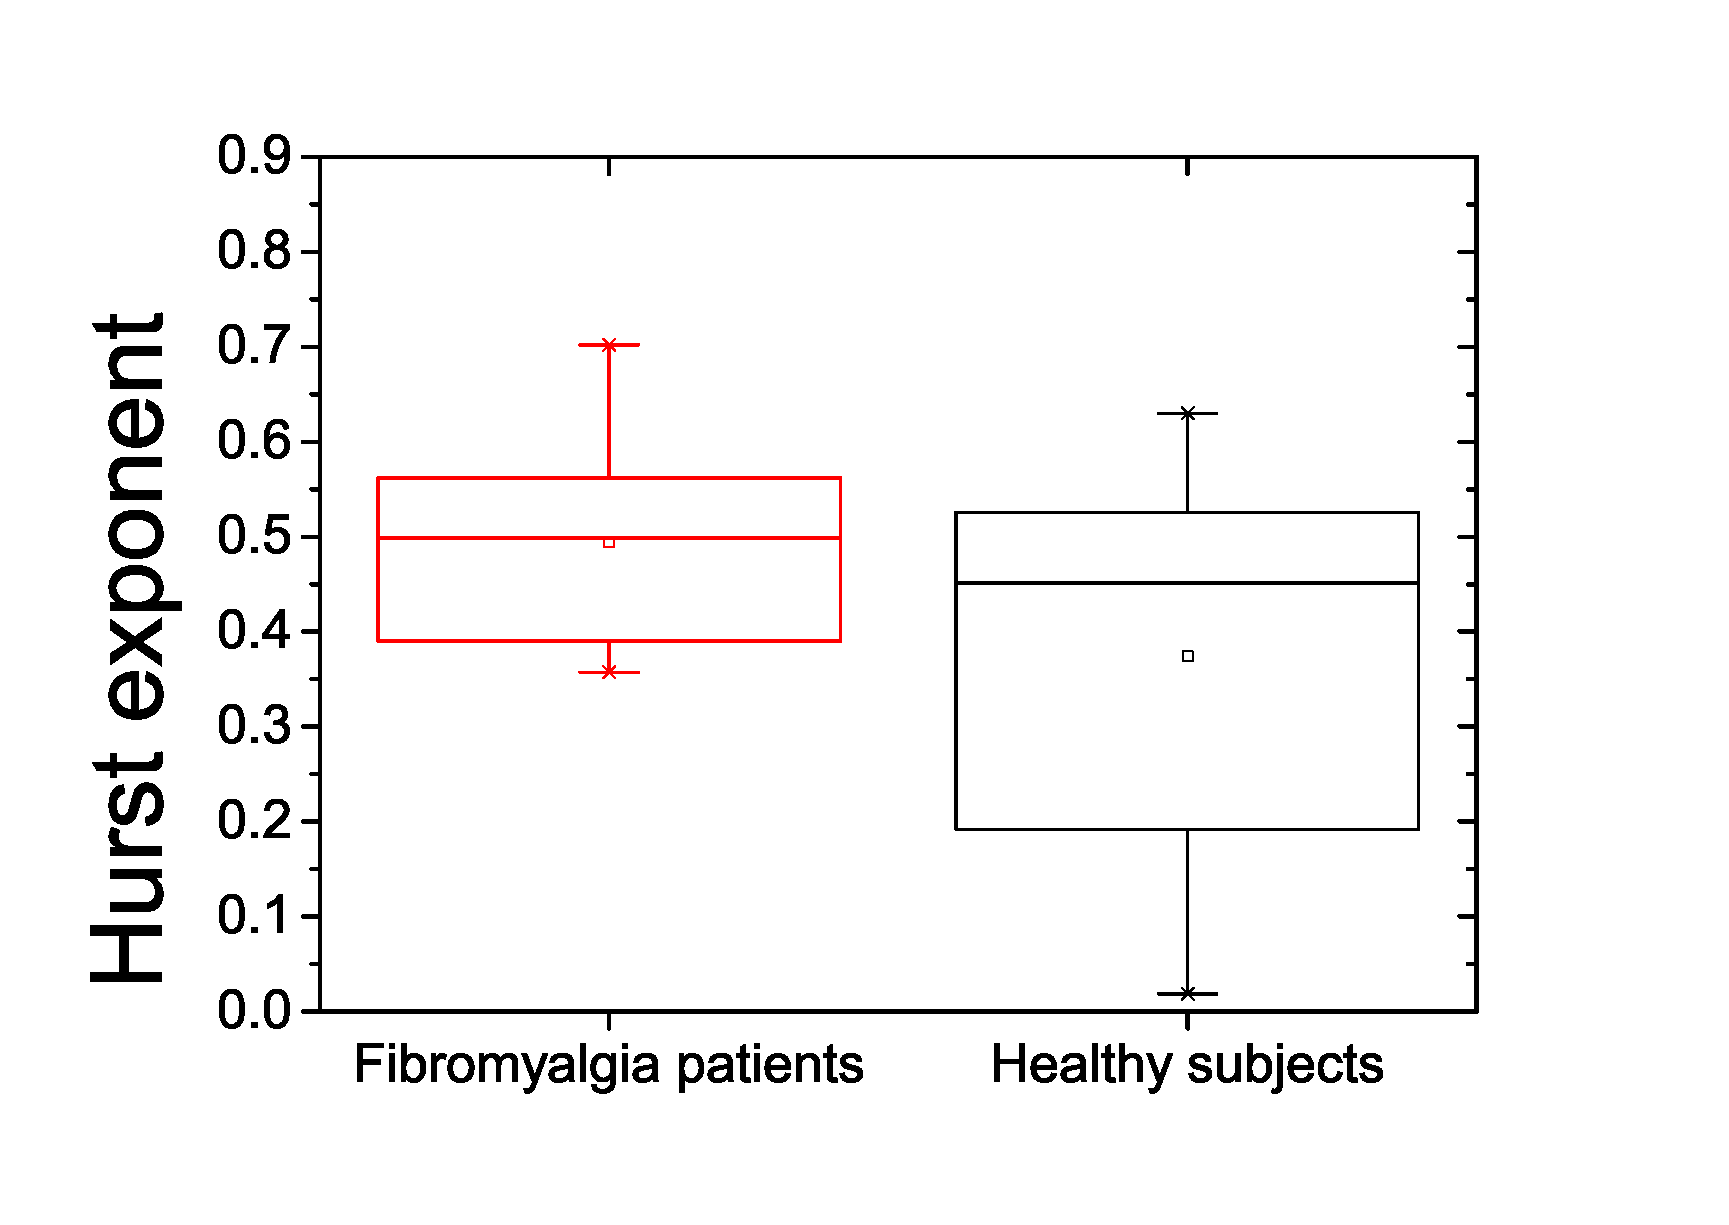
\includegraphics[width=6in]{hurst_ap}
\end{center}
\caption{
{\bf Fluxogram.} Boxplot of Hurst exponents of antero-posterior body sway for FM patients (in red) and pain-free control subjects (in black).
}
\label{fig:HurstPosteriorAnterior}
\end{figure}
\newpage

\begin{figure}[!ht]
\begin{center}
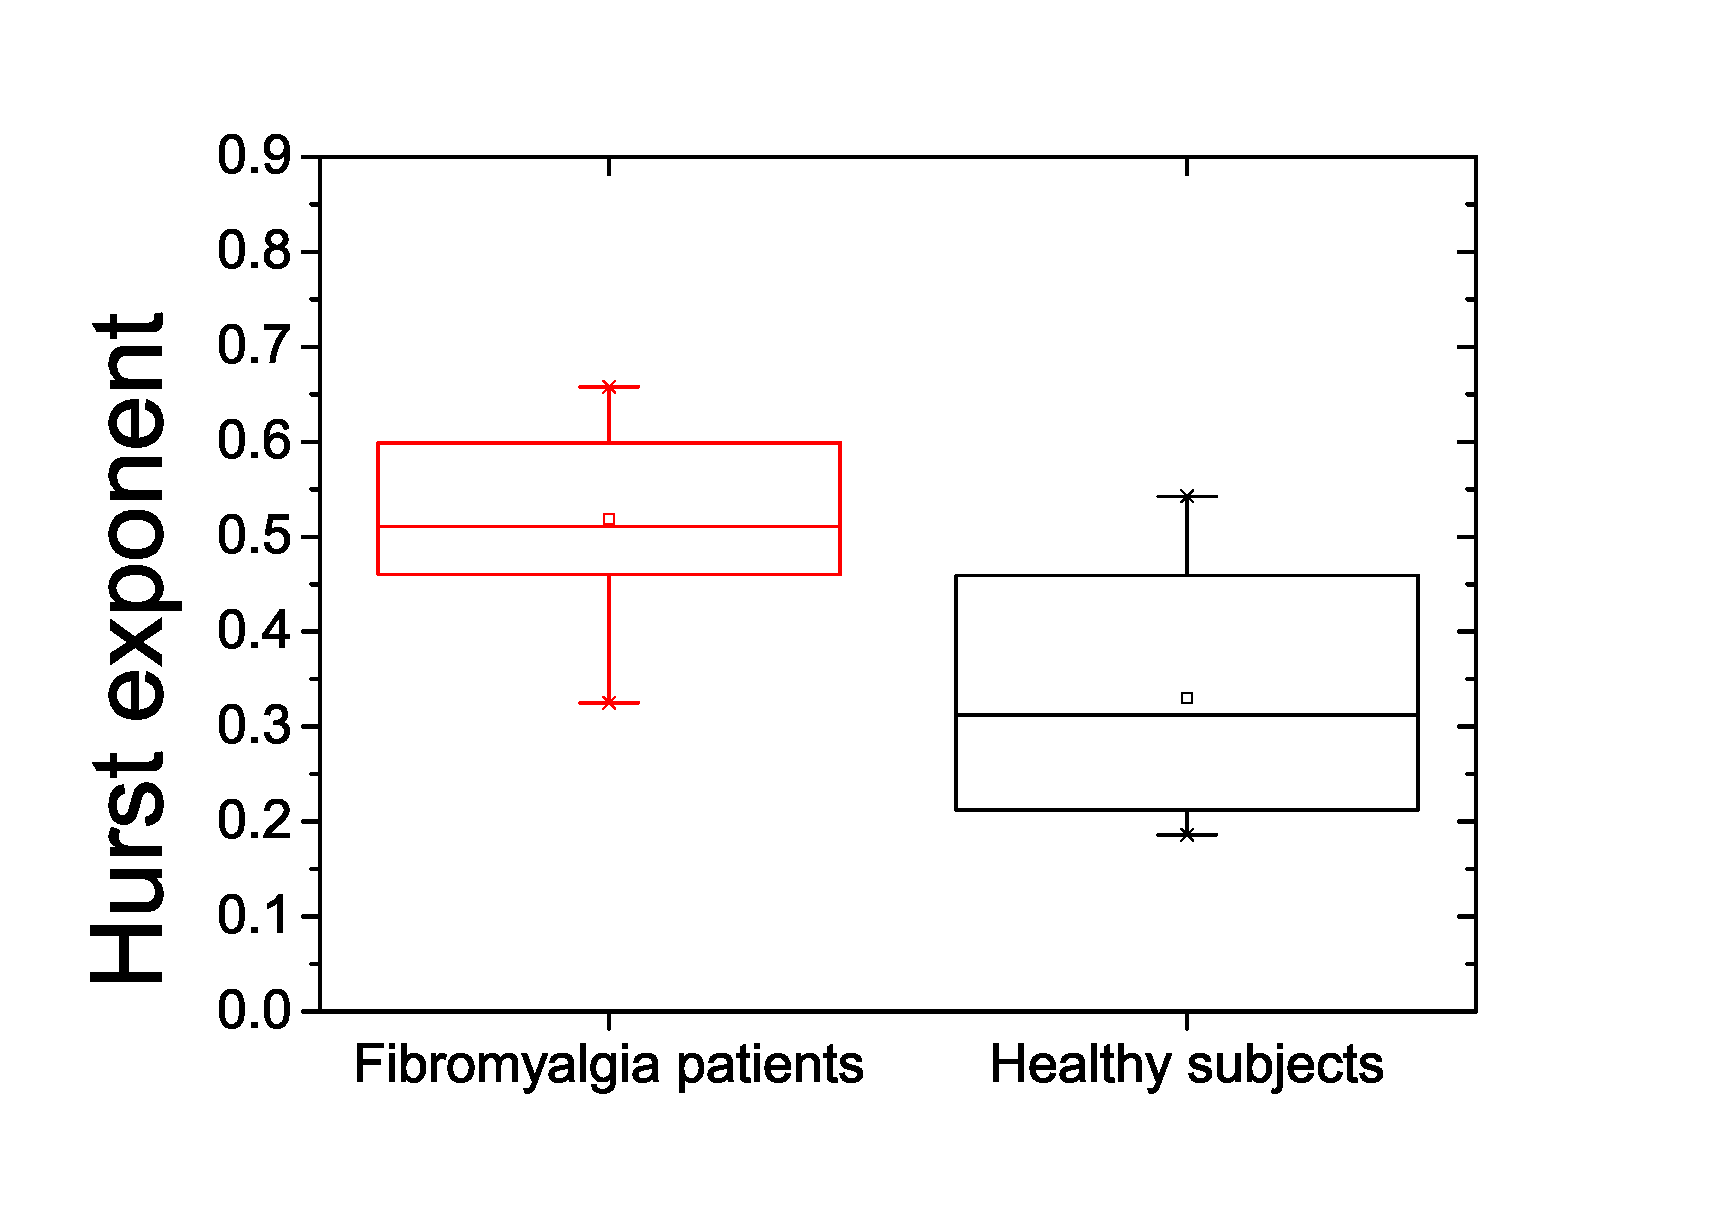
\includegraphics[width=6in]{hurst_ml}
\end{center}
\caption{
{\bf Fluxogram.} Boxplot of Hurst exponents of medial-lateral body sway for FM patients (in red) and pain-free control subjects (in black).
}
\label{fig:HurstMedialLateral}
\end{figure}

%\begin{figure}[!ht]
%\begin{center}
%%\includegraphics[width=4in]{figure_name.2.eps}
%\end{center}
%\caption{
%{\bf Bold the first sentence.}  Rest of figure 2  caption.  Caption 
%should be left justified, as specified by the options to the caption 
%package.
%}
%\label{Figure_label}
%\end{figure}

%\vspace{1cm}
\newpage

\section*{Tables}
\begin{table}[ht]
\caption{Demographic characteristics of participants. It has been considered a 95\% confidence interval for all Kolmogorov-Smirnov test.}
\begin{tabular}{lccc}
	\hline 
	& Fibromyalgia & Pain-free  & Kolmogorov-Smirnov \\ \\
	 & patients & controls & test for inequality \\ \\
 	 & N = 17 & N = 17 & (F, p-value)
 \\ \\ \hline
 Age (yrs)	& $49.06 \pm 8.4$ &	$43.2 \pm 8.3$ &	$(0.46, 0.07)$
  \\ \\ 
 Weight (Kg)	& $69.9 \pm 10.9$ &	$63.6 \pm 10.9$ &	$(0.29, 0.45)$
   \\ \\ 
 Height (cm)	& $159.9 \pm 8.61$ &	$163.82 \pm 7.09$ &	$(0.29, 0.45)$
   \\ \\ 
 Body Mass Index	& $27.3 \pm 3.8$ &	$23.7 \pm 3.9$ &	$(0.52, 0.02)^\ast$
    \\ \\ 
FM History (yrs)	& $7.5 \pm 5.5$ &	-- &
 \\ \hline
Values are mean $\pm$ standard deviation\\
$*$ p$<$0.05
\end{tabular}
\label{tab:demography}
\end{table}

\newpage
\begin{table}[ht]
\caption{List of medication in FM participants}
\begin{tabular}{lc}
	\hline 
	& Number of Patients  \\ \\ \hline
%%ANTIDEPRESSANTS
 \textbf{ANTIDEPRESSANTS}  & \\ \\
    \emph{Selective serotonin reuptake inhibitor}  & 11 (64.7\%)  \\ \\ 
    
    \emph{Melatonergic receptor agonist (MT1 and MT2) and selective }  &   \\ 
\hspace{1.0cm} \emph{antagonist of the serotonergic}  & 2 (11.7\%)  \\ \\

    \emph{Non-selective monoamine reuptake inhibitors}  &   1 (5.9\%)  \\ \\ \\

%%ANALGESICS
   \textbf{ANALGESICS}  & \\ \\
    \emph{Clonixin, Tramadol hydrochloride, Paracetamol, Magnesium}  & \\ 
    \hspace{1.0cm} \emph{metamizol}  & 11 (64.7\%)  \\ \\ \\

%%ANXIOLYTICS    
    \textbf{ANXIOLYTICS}  & \\ \\
    \emph{Diazepam, Lorazepam, Alprazolam}  & 6 (35.3\%)  \\ \\ \\

%%ANTIFLAMATORY
   \textbf{ANTIINFLAMATORY AND ANTIRHEUMATIC, NON-STEROIDS}  & \\ \\
    \emph{Celecoxib, Etoricoxib, Dexketoprofen, Ibuprofen, Naproxen,}  & \\ 
    \hspace{1.0cm} \emph{Piroxicam}  & 8 (47\%) \\ \\
    \hline
\end{tabular}
\label{tab:medication}
\end{table}
\newpage
\begin{table}[ht]
\caption{Patients records for each subscale in Fibromyalgia Impact Questionnaire (FIQ). Values are mean $\pm$ standard deviation}
\begin{tabular}{lcc}
	\hline 
	Fibromyalgia Impact Questionnaire & & Fibromyalgia patients \\ \\
 	          (FIQ) &  & N = 17\\ \\ 
 	\hline 
\hspace{0.4cm} Physical impairment (0-3)        &       &  $1.6  \pm 0.8$\\ \\
\hspace{0.4cm} Feel good (0-7)                  &        & $5.7  \pm 1.9\\ \\
\hspace{0.4cm} Work missed (0-7)                &        & $2.3  \pm 2.3$\\ \\
\hspace{0.4cm} Do work (10 cm VAS)              &        & $8.1  \pm 2.0$\\ \\
\hspace{0.4cm} Pain (10 cm VAS)                 &        & $8.1  \pm 1.9$\\ \\
\hspace{0.4cm} Fatigue (10 cm VAS)              &        & $8.9  \pm 1.9$\\ \\
\hspace{0.4cm} Rested (10 cm VAS)               &        & $8.3  \pm 3.0$\\ \\
\hspace{0.4cm} Stiffness (10 cm VAS)            &        & $7.6  \pm 3.0$\\ \\
\hspace{0.4cm} Anxiety (10 cm VAS)              &        & $7.7  \pm 2.8$\\ \\
\hspace{0.4cm} Depression (10 cm VAS)           &        & $7.0  \pm 3.4$\\ \\
\hspace{0.4cm} Total FIQ score (0-100)          &      & $71.7  \pm 16.8$\\ \\ \hline
\end{tabular}
\label{tab:FIQ}
\end{table}
\newpage
\begin{table}[ht]
\caption{Mean and standard deviations of gait parameters during motor performance in fibromyalgia patients and pain-free controls. It has been considered a 95\% confidence interval for both Student’s t and Kolmogorov-Smirnov tests.}
\begin{tabular}{lccl}
	\hline 
	& Fibromyalgia & Pain-free  & Test for\\ \\
	 & patients & controls &  inequality\\ \\
 	 & N = 17 & N = 17 &  of datasets\\ \\ \hline
\emph{Standardized motor function tests}  &  &  &  \\ \\
\hspace{0.3cm} TUG (secs)  & $16.5 \pm 3.9$ & $8.2 \pm 1.0$ & $t(16) =8.41,~p < .001$ \\ \\
\hspace{0.3cm} 6MWT (m)  & $168.6 \pm 45.2$ & $334.0 \pm 58.7$ & $t(16) =-9.20,~p < .001$ \\ \\
\hspace{0.3cm} Berg scale for risk of falls (0--56)  & $44.9 \pm 5.7$ & $55.41 \pm 0.61$ & $ks(16) =-11.99,~p < .001$\\ \\  
\hspace{0.3cm} Perceived effort after TUG (4--20)  & $11.5 \pm 2.2$ & $4.4 \pm 0.6$ & $ks(16) = 12.74,~p < .001$ \\ \\
\hspace{0.3cm} Perceived effort after 6MWT (4--20)  & $13.8 \pm 3.5$ & $9.4 \pm 3.1$ & $ks(16) = 3.85,~p < .001$ \\ \\ \hline

\emph{Gait parameters}  &  &  &  \\ \\
\hspace{0.3cm} Gait velocity (cm/sec)  & $68.0 \pm 17.2$ & $98.8 \pm 12.3$ & $t(16) =-8.65,~p < .001$ \\ \\  
\hspace{0.3cm} Gait duration (sec)  & $4.6 \pm 1.5$ & $2.7 \pm 0.3$ & $t(16)=5.95,~p < .001$ \\ \\
\hspace{0.3cm} Cadence (steps/min)  & $94.3 \pm 11.3$ & $115.2 \pm 11.3$ & $t(16)=-6.45, ~p < .001$ \\ \\
\hspace{0.3cm} Stride Length (cm)  & $69.3 \pm 14.3$ & $99.2 \pm 12.9$ & $t(16)=-5.39, ~p < .01$ \\ \\
\hspace{0.3cm} Step Length (cm)  & $58.6 \pm 10.5$ & $79.7 \pm 8.6$ & $t(16)=-5.06,~p < .01$ \\ \\
\hspace{0.3cm} Single support (\%)  & $57.1 \pm 7.6$ & $66.2 \pm 4.0$ & $t(16)=-4.50,~p < .01$ \\ \\
\hspace{0.3cm} Swing phase (\%)  & $36.3 \pm 3.0$ & $39.8 \pm 1.5$ & $t(16)=4.62,~p < .01$ \\ \\
\hline
Values are mean $\pm$ standard deviation\\
\end{tabular}
\label{tab:gait}
\end{table}
\newpage
\begin{table}[ht].\caption{Mean and standard deviations of Anterior-Posterior (AP) and Medial-Lateral (ML) balance parameters during motor performance in fibromyalgia patients and pain-free controls. It has been considered a 95\% confidence interval for all Student’s t-test.}
\begin{tabular}{lccl}
	\hline 
	& Fibromyalgia & Pain-free  & Student's t-test for\\ \\
	 & patients & controls &  inequality of datasets\\ \\
 	 & N = 15 & N = 15 & (F, p-value) \\ \\ \hline
\emph{Balance parameters}  &  &  &  \\ \\
\hspace{0.3cm} AP Body sway (cm)  & $1.48 \pm 4.81$ & $0.32 \pm 0.73$ & $(t=-15.25,~p < .001)$ \\ \\  
\hspace{0.3cm} ML Body sway (cm)  & $-0.81 \pm 6.11$ & $0.67 \pm 1.13$ & $(t=-10.40,~p < .001)$ \\ \\ 
\hspace{0.3cm} AP Hurst exponent & $0.50 \pm 0.10$ & $0.37 \pm 0.19$ & $(t= 2.31,~p < .05)$ \\ \\
\hspace{0.3cm} ML Hurst exponent & $0.52 \pm 0.09$ & $0.33 \pm 0.12$ & $(t= 4.74,~p < .001)$ \\ \\ \hline
Values are mean $\pm$ standard deviation\\
\end{tabular}
\label{tab:balance}
\end{table}

\newpage
\begin{landscape}
\begin{table}[ht]
\caption{Pearson correlations of FIQ subscales and sleep quality with performance parameters on standard motor function tasks, as well as  with movement parameters extracted from video recordings during performance on gait and balance tasks in fibromyalgia patients. Confidence interval CI=0.95. Statistically significant correlations with \textbf{$^\ast$} indicating $p < 0.05$ and \textbf{$^{\ast\ast}$} $p< 0.01$. }
\begin{tabular}{lccccc}
        \hline
        & \multicolumn{4}{c}{\emph{\textbf{FIQ subscales}}}\\ \\
 & \emph{\textbf{Pain}} & \emph{\textbf{Depression}} & \emph{\textbf{Anxiety}} & \emph{\textbf{Fatigue}} & \emph{\textbf{Stiffness}} \\ \\ \hline
\emph{Standardized motor function tests}  & & & & & \\ \\
\hspace{0.3cm} Berg scale for risk of falls (0--56)  & -0.53\textbf{$^\ast$} & -0.53\textbf{$^\ast$} & -0.63\textbf{$^{\ast\ast}$} & - & -\\ \\
\
\hspace{0.3cm} TUG (secs)  & 0.47\textbf{$^\ast$} & 0.54\textbf{$^\ast$}  & - & - & 0.50\textbf{$^\ast$} \\ \\
\hspace{0.3cm} Perceived effort after TUG (4--20)  & - & - & - & - & - \\ \\
\hspace{0.3cm} 6MWT (m)  & - & - & - & - & - \\ \\
\hspace{0.3cm} Perceived effort after 6MWT (4--20)  & - & - & - & - & 0.63\textbf{$^\ast$} \\ \\ \hline

\emph{Gait parameters}  &  & & & &   \\ \\
\hspace{0.3cm} Gait velocity (cm/sec)  & -0.50\textbf{$^\ast$} & - & - & - & - \\ \\
\hspace{0.3cm} Gait duration (sec)  & 0.50\textbf{$^\ast$} & - & - & - & - \\ \\
\hspace{0.3cm} Cadence (steps/min)  &  - & - & - & - & - \\ \\
\hspace{0.3cm} Stride Length (cm)  & -0.55\textbf{$^\ast$} & - & - & - & - \\ \\
\hspace{0.3cm} Step Length (cm)  & -0.56\textbf{$^\ast$} & - & - & - & -0.29\textbf{$^\ast$} \\ \\
\hspace{0.3cm} Single support (\%)  & - & - & - & -0.52\textbf{$^\ast$} & -0.48\textbf{$^\ast$}\\ \\
\hspace{0.3cm} Swing phase (\%)  & - & - & - & -0.51\textbf{$^\ast$} & -0.48\textbf{$^\ast$} \\ \\
\hline
\end{tabular}
\label{tab:pearson}
\end{table}
\end{landscape}


%\begin{table}[!ht]
%\caption{
%\bf{Table title}}
%\begin{tabular}{|c|c|c|}
%table information
%\end{tabular}
%\begin{flushleft}Table caption
%\end{flushleft}
%\label{tab:label}
% \end{table}
\end{document}